 \documentclass{article}
\usepackage[utf8]{inputenc}
\usepackage[a4paper, total={7in, 10in}]{geometry}
\usepackage{braket}
\usepackage{xcolor}
\usepackage{amsmath}
\usepackage{amssymb}
\usepackage{amsfonts}
\usepackage{graphicx}
\usepackage{svg}
\usepackage{float}
\usepackage{tikz}
\usepackage[ruled,vlined]{algorithm2e}
\usepackage{multicol}
\usepackage[backend=biber,style=alphabetic,sorting=ynt]{biblatex}
\usepackage{xcolor}
%\addbibresource{sample.bib} %Import the bibliography file

\newcommand{\commentt}[1]{\textcolor{blue}{ \textbf{[COMMENT]} #1}}
\newcommand{\ctt}[1]{\commentt{#1}}
\newcommand{\prb}[1]{ \mathbf{Pr} \left[ {#1} \right]}
\newcommand{\onotation}[1]{\(\mathcal{O} \left( {#1}  \right) \)}
\newcommand{\ona}[1]{\onotation{#1}}
\newcommand{\PSI}{{\ket{\psi}}}
\newcommand{\LESn}{\ket{\psi_n}}
\newcommand{\LESa}{\ket{\phi_n}}
\newcommand{\LESs}{\frac{1}{\sqrt{n}}\sum_{i}{\ket{\left(0^{i}10^{n-i}\right)^{n}}}}
\newcommand{\Hn}{\mathcal{H}_{n}}
\newcommand{\Ep}{\frac{1}{\sqrt{2^n}}\sum^{2^n}_{x}{ \ket{xx}}}
\newcommand{\HON}{\ket{\psi_{\text{honest}}}}
\newcommand{\Lemma}{\paragraph{Lemma.}}


\setlength{\columnsep}{0.6cm}

\newcommand{\Gz}{ G_{z}^{\delta} } 

\begin{document}

\title{Quantum LTC With Positive Rate}
\author{David Ponarovsky}
\maketitle
%\begin{multicols*}{2}
\newcommand{ \Hw }{ \delta\Delta -\Delta^{\frac{1}{2}-\varepsilon}/\delta  }
	\newcommand{ \Nw }{ \Delta^{\frac{3}{2}-\varepsilon}} 
	  \newcommand{ \Gu } { \Gamma^{\cup} }
	  \newcommand{ \Guq } { \Gamma^{\cup, \square} }

    	\newcommand{ \Gsa } {\Gamma_{\square_{1}} }
	\newcommand{ \Gsb } {\Gamma_{\square_{2}} }
        \newcommand{ \Aa } { C_{A_{1}}}  
	\newcommand{ \Ab } { C_{A_{2}}}
	\newcommand{ \Ac } { C_{A_{3}}}
	\newcommand{ \Aab } { \Aa \otimes \Ab } 
	\newcommand{ \Aac } { \Aa \otimes \Ac }
	\newcommand{ \Aabc } { \Aa \otimes \Ab \otimes \Ac }
	\newcommand{ \Aabp } { \Aa^{\perp} \otimes \Ab^{\perp} } 
	\newcommand{ \Aacp } { \Aa^{\perp} \otimes \Ac^{\perp} }
	\newcommand{ \Aabcp } { \Aa^{\perp} \otimes \Ab^{\perp} \otimes \Ac^{\perp} }
	\newcommand{ \Aabpp } { \left( \Aabp \right)^\perp } 
	\newcommand{ \Aacpp } { \left( \Aacp \right)^\perp }
	\newcommand{ \Aabcpp } { \left( \Aabcp \right)^\perp }
	\newcommand{ \YY } {  y_{1}y_{2}^{\top} }
	\newcommand{ \ZZ } {  z_{1}z_{2}^{\top} } 
	\newcommand{ \TT } { \tilde{\tau} } 


  \paragraph{preamble.} preamble.  
  \begin{figure}[H]
            %\label{fig:square}
            \begin{center}
            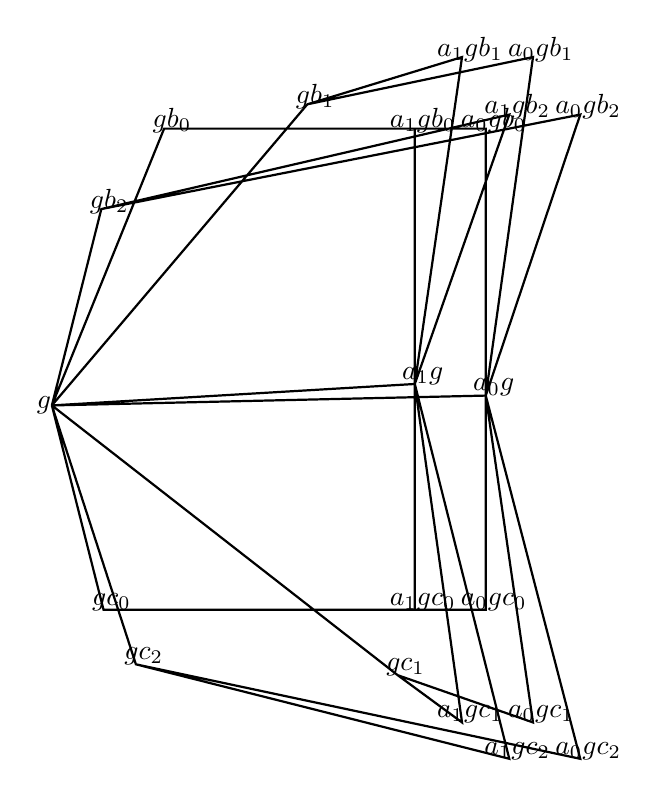
\begin{tikzpicture}
            \draw[thick](0,0)(0,0) -- (1.4255136291753252,3.515325204588676) -- (5.510402982634022,3.515325204588676) -- (5.510402982634022,0.12499050095569095) -- (0,0)
(0,0) -- (3.2445778281487545,3.8241458070304675) -- (6.110402982634022,4.424145807030468) -- (5.510402982634022,0.12499050095569095) -- (0,0)
(0,0) -- (0.6280420466015907,2.493817375601831) -- (6.710402982634022,3.6938173756018307) -- (5.510402982634022,0.12499050095569095) -- (0,0)
(0,0) -- (1.4255136291753252,3.515325204588676) -- (4.609120751916487,3.515325204588676) -- (4.609120751916487,0.2724037129657107) -- (0,0)
(0,0) -- (3.2445778281487545,3.8241458070304675) -- (5.209120751916487,4.424145807030468) -- (4.609120751916487,0.2724037129657107) -- (0,0)
(0,0) -- (0.6280420466015907,2.493817375601831) -- (5.809120751916487,3.6938173756018307) -- (4.609120751916487,0.2724037129657107) -- (0,0)
(0,0) -- (0.6557330193015071,-2.593566251458001) -- (5.510402982634022,-2.593566251458001) -- (5.510402982634022,0.12499050095569095) -- (0,0)
(0,0) -- (4.3920278615301696,-3.4259419407174) -- (6.110402982634022,-4.0259419407173995) -- (5.510402982634022,0.12499050095569095) -- (0,0)
(0,0) -- (1.0671958706645683,-3.287761330112935) -- (6.710402982634022,-4.487761330112935) -- (5.510402982634022,0.12499050095569095) -- (0,0)
(0,0) -- (0.6557330193015071,-2.593566251458001) -- (4.609120751916487,-2.593566251458001) -- (4.609120751916487,0.2724037129657107) -- (0,0)
(0,0) -- (4.3920278615301696,-3.4259419407174) -- (5.209120751916487,-4.0259419407173995) -- (4.609120751916487,0.2724037129657107) -- (0,0)
(0,0) -- (1.0671958706645683,-3.287761330112935) -- (5.809120751916487,-4.487761330112935) -- (4.609120751916487,0.2724037129657107) -- (0,0)
;
\node at (5.610402982634022,3.615325204588676) {$ a_{ 0  } gb_{ 0 } $};
\node at (6.2104029826340215,4.524145807030467) {$ a_{ 0  } gb_{ 1 } $};
\node at (6.810402982634022,3.7938173756018307) {$ a_{ 0  } gb_{ 2 } $};
\node at (4.709120751916487,3.615325204588676) {$ a_{ 1  } gb_{ 0 } $};
\node at (5.3091207519164865,4.524145807030467) {$ a_{ 1  } gb_{ 1 } $};
\node at (5.909120751916487,3.7938173756018307) {$ a_{ 1  } gb_{ 2 } $};
\node at (5.610402982634022,-2.493566251458001) {$ a_{ 0  } gc_{ 0 } $};
\node at (6.2104029826340215,-3.9259419407173994) {$ a_{ 0  } gc_{ 1 } $};
\node at (6.810402982634022,-4.3877613301129355) {$ a_{ 0  } gc_{ 2 } $};
\node at (4.709120751916487,-2.493566251458001) {$ a_{ 1  } gc_{ 0 } $};
\node at (5.3091207519164865,-3.9259419407173994) {$ a_{ 1  } gc_{ 1 } $};
\node at (5.909120751916487,-4.3877613301129355) {$ a_{ 1  } gc_{ 2 } $};
\node at (-0.1,0) {$ g $};
\node at (5.610402982634022,0.22499050095569095) {$ a_{ 0 }g $};
\node at (4.709120751916487,0.37240371296571073) {$ a_{ 1 }g $};
\node at (1.5255136291753253,3.615325204588676) {$ gb_{ 0 } $};
\node at (3.3445778281487546,3.9241458070304676) {$ gb_{ 1 } $};
\node at (0.7280420466015907,2.593817375601831) {$ gb_{ 2 } $};
\node at (0.755733019301507,-2.493566251458001) {$ gc_{ 0 } $};
\node at (4.492027861530169,-3.3259419407174) {$ gc_{ 1 } $};
\node at (1.1671958706645684,-3.187761330112935) {$ gc_{ 2 } $};

            \end{tikzpicture}
            \end{center}
            \caption{Square of the complex, with edges $(g,ag), (agb, gb) \in E_A,
            (g,gb), (agb, ag) \in E_B.$ \label{fig:square}
            }
            \end{figure}
 \begin{figure}[H]
            %\label{fig:square}
            \begin{center}
            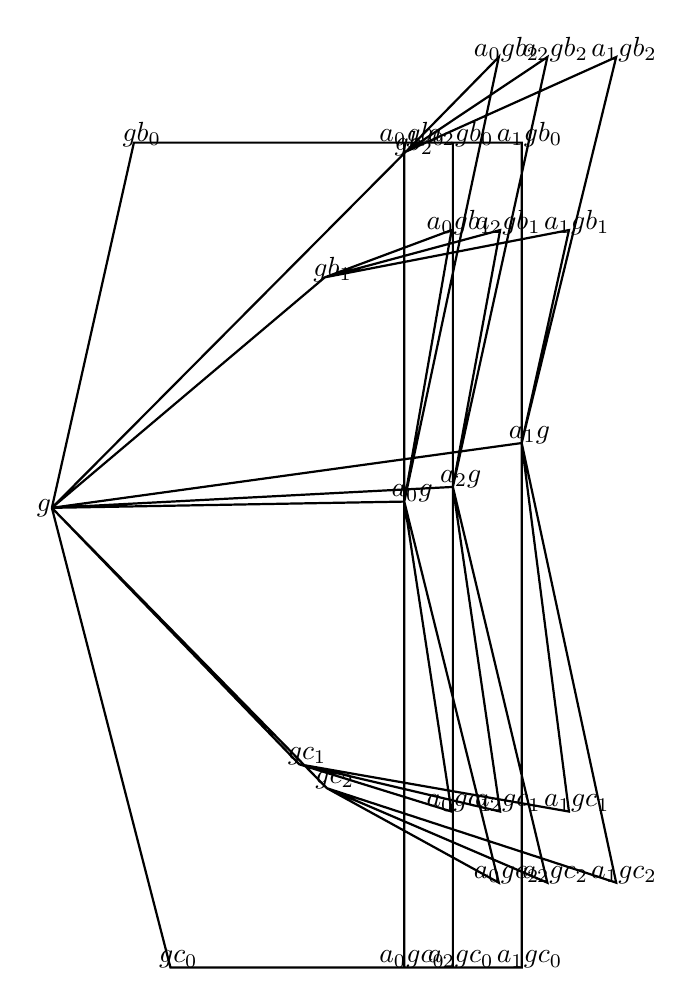
\begin{tikzpicture}
            \draw[thick](0,0)(0,0) -- (1.041941977290004,4.638164822204152) -- (4.475678542348576,4.638164822204152) -- (4.475678542348576,0.07921977522295402) -- (0,0)
(0,0) -- (3.466537573490305,2.9273399040617822) -- (5.075678542348576,3.5273399040617823) -- (4.475678542348576,0.07921977522295402) -- (0,0)
(0,0) -- (4.498120282567632,4.524658908606837) -- (5.675678542348576,5.724658908606838) -- (4.475678542348576,0.07921977522295402) -- (0,0)
(0,0) -- (1.041941977290004,4.638164822204152) -- (5.966799046886828,4.638164822204152) -- (5.966799046886828,0.8229149924695285) -- (0,0)
(0,0) -- (3.466537573490305,2.9273399040617822) -- (6.566799046886827,3.5273399040617823) -- (5.966799046886828,0.8229149924695285) -- (0,0)
(0,0) -- (4.498120282567632,4.524658908606837) -- (7.166799046886828,5.724658908606838) -- (5.966799046886828,0.8229149924695285) -- (0,0)
(0,0) -- (1.041941977290004,4.638164822204152) -- (5.092708840590738,4.638164822204152) -- (5.092708840590738,0.2653638179884247) -- (0,0)
(0,0) -- (3.466537573490305,2.9273399040617822) -- (5.692708840590738,3.5273399040617823) -- (5.092708840590738,0.2653638179884247) -- (0,0)
(0,0) -- (4.498120282567632,4.524658908606837) -- (6.2927088405907385,5.724658908606838) -- (5.092708840590738,0.2653638179884247) -- (0,0)
(0,0) -- (1.5063090880439018,-5.838860753739607) -- (4.475678542348576,-5.838860753739607) -- (4.475678542348576,0.07921977522295402) -- (0,0)
(0,0) -- (3.1416807687932735,-3.257146443101021) -- (5.075678542348576,-3.857146443101021) -- (4.475678542348576,0.07921977522295402) -- (0,0)
(0,0) -- (3.4924974483719495,-3.560454824539024) -- (5.675678542348576,-4.760454824539024) -- (4.475678542348576,0.07921977522295402) -- (0,0)
(0,0) -- (1.5063090880439018,-5.838860753739607) -- (5.966799046886828,-5.838860753739607) -- (5.966799046886828,0.8229149924695285) -- (0,0)
(0,0) -- (3.1416807687932735,-3.257146443101021) -- (6.566799046886827,-3.857146443101021) -- (5.966799046886828,0.8229149924695285) -- (0,0)
(0,0) -- (3.4924974483719495,-3.560454824539024) -- (7.166799046886828,-4.760454824539024) -- (5.966799046886828,0.8229149924695285) -- (0,0)
(0,0) -- (1.5063090880439018,-5.838860753739607) -- (5.092708840590738,-5.838860753739607) -- (5.092708840590738,0.2653638179884247) -- (0,0)
(0,0) -- (3.1416807687932735,-3.257146443101021) -- (5.692708840590738,-3.857146443101021) -- (5.092708840590738,0.2653638179884247) -- (0,0)
(0,0) -- (3.4924974483719495,-3.560454824539024) -- (6.2927088405907385,-4.760454824539024) -- (5.092708840590738,0.2653638179884247) -- (0,0)
;
\node at (4.575678542348576,4.738164822204151) {$ a_{ 0  } gb_{ 0 } $};
\node at (5.175678542348575,3.6273399040617824) {$ a_{ 0  } gb_{ 1 } $};
\node at (5.775678542348576,5.824658908606837) {$ a_{ 0  } gb_{ 2 } $};
\node at (6.066799046886827,4.738164822204151) {$ a_{ 1  } gb_{ 0 } $};
\node at (6.666799046886827,3.6273399040617824) {$ a_{ 1  } gb_{ 1 } $};
\node at (7.2667990468868275,5.824658908606837) {$ a_{ 1  } gb_{ 2 } $};
\node at (5.192708840590738,4.738164822204151) {$ a_{ 2  } gb_{ 0 } $};
\node at (5.792708840590738,3.6273399040617824) {$ a_{ 2  } gb_{ 1 } $};
\node at (6.392708840590738,5.824658908606837) {$ a_{ 2  } gb_{ 2 } $};
\node at (4.575678542348576,-5.7388607537396075) {$ a_{ 0  } gc_{ 0 } $};
\node at (5.175678542348575,-3.757146443101021) {$ a_{ 0  } gc_{ 1 } $};
\node at (5.775678542348576,-4.660454824539024) {$ a_{ 0  } gc_{ 2 } $};
\node at (6.066799046886827,-5.7388607537396075) {$ a_{ 1  } gc_{ 0 } $};
\node at (6.666799046886827,-3.757146443101021) {$ a_{ 1  } gc_{ 1 } $};
\node at (7.2667990468868275,-4.660454824539024) {$ a_{ 1  } gc_{ 2 } $};
\node at (5.192708840590738,-5.7388607537396075) {$ a_{ 2  } gc_{ 0 } $};
\node at (5.792708840590738,-3.757146443101021) {$ a_{ 2  } gc_{ 1 } $};
\node at (6.392708840590738,-4.660454824539024) {$ a_{ 2  } gc_{ 2 } $};
\node at (-0.1,0) {$ g $};
\node at (4.575678542348576,0.17921977522295401) {$ a_{ 0 }g $};
\node at (6.066799046886827,0.9229149924695285) {$ a_{ 1 }g $};
\node at (5.192708840590738,0.36536381798842466) {$ a_{ 2 }g $};
\node at (1.1419419772900041,4.738164822204151) {$ gb_{ 0 } $};
\node at (3.566537573490305,3.0273399040617823) {$ gb_{ 1 } $};
\node at (4.598120282567631,4.624658908606837) {$ gb_{ 2 } $};
\node at (1.606309088043902,-5.7388607537396075) {$ gc_{ 0 } $};
\node at (3.2416807687932736,-3.1571464431010208) {$ gc_{ 1 } $};
\node at (3.5924974483719496,-3.460454824539024) {$ gc_{ 2 } $};

            \end{tikzpicture}
            \end{center}
            \caption{Square of the complex, with edges $(g,ag), (agb, gb) \in E_A,
            (g,gb), (agb, ag) \in E_B.$ \label{fig:square}
            }
            \end{figure}
 \begin{figure}[H]
            %\label{fig:square}
            \begin{center}
            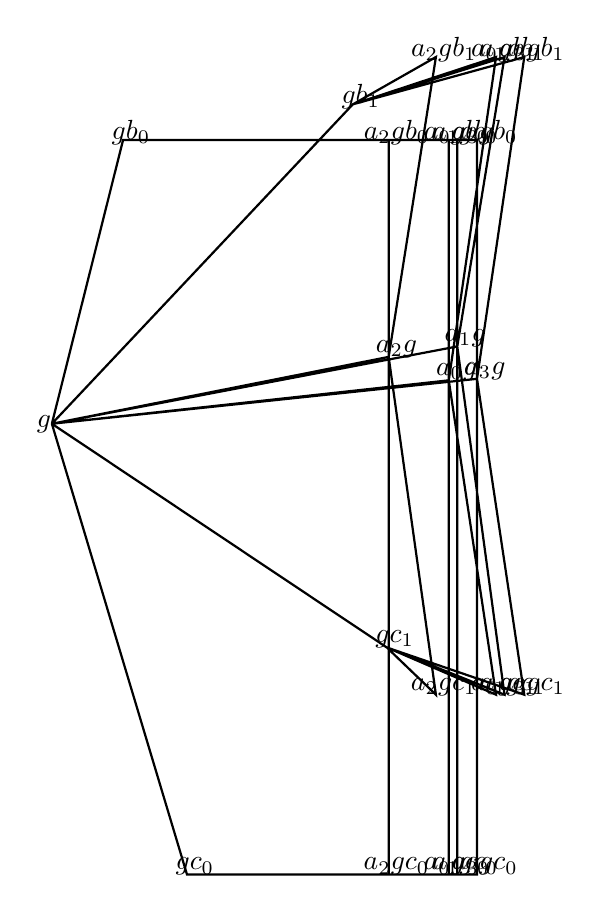
\begin{tikzpicture}
            \draw[thick](0,0)(0,0) -- (0.9043957076994952,3.603846310776421) -- (5.040566027944072,3.603846310776421) -- (5.040566027944072,0.5514376465734241) -- (0,0)
(0,0) -- (3.82271319442105,4.056905343936612) -- (5.640566027944072,4.656905343936612) -- (5.040566027944072,0.5514376465734241) -- (0,0)
(0,0) -- (0.9043957076994952,3.603846310776421) -- (5.148623474627834,3.603846310776421) -- (5.148623474627834,0.9819079214209311) -- (0,0)
(0,0) -- (3.82271319442105,4.056905343936612) -- (5.748623474627833,4.656905343936612) -- (5.148623474627834,0.9819079214209311) -- (0,0)
(0,0) -- (0.9043957076994952,3.603846310776421) -- (4.277220749193093,3.603846310776421) -- (4.277220749193093,0.8492868998103268) -- (0,0)
(0,0) -- (3.82271319442105,4.056905343936612) -- (4.877220749193093,4.656905343936612) -- (4.277220749193093,0.8492868998103268) -- (0,0)
(0,0) -- (0.9043957076994952,3.603846310776421) -- (5.399425047230509,3.603846310776421) -- (5.399425047230509,0.5705091093243199) -- (0,0)
(0,0) -- (3.82271319442105,4.056905343936612) -- (5.999425047230509,4.656905343936612) -- (5.399425047230509,0.5705091093243199) -- (0,0)
(0,0) -- (1.716074273651692,-5.724129583478823) -- (5.040566027944072,-5.724129583478823) -- (5.040566027944072,0.5514376465734241) -- (0,0)
(0,0) -- (4.253318927235555,-2.840883391110042) -- (5.640566027944072,-3.440883391110042) -- (5.040566027944072,0.5514376465734241) -- (0,0)
(0,0) -- (1.716074273651692,-5.724129583478823) -- (5.148623474627834,-5.724129583478823) -- (5.148623474627834,0.9819079214209311) -- (0,0)
(0,0) -- (4.253318927235555,-2.840883391110042) -- (5.748623474627833,-3.440883391110042) -- (5.148623474627834,0.9819079214209311) -- (0,0)
(0,0) -- (1.716074273651692,-5.724129583478823) -- (4.277220749193093,-5.724129583478823) -- (4.277220749193093,0.8492868998103268) -- (0,0)
(0,0) -- (4.253318927235555,-2.840883391110042) -- (4.877220749193093,-3.440883391110042) -- (4.277220749193093,0.8492868998103268) -- (0,0)
(0,0) -- (1.716074273651692,-5.724129583478823) -- (5.399425047230509,-5.724129583478823) -- (5.399425047230509,0.5705091093243199) -- (0,0)
(0,0) -- (4.253318927235555,-2.840883391110042) -- (5.999425047230509,-3.440883391110042) -- (5.399425047230509,0.5705091093243199) -- (0,0)
;
\node at (5.140566027944072,3.703846310776421) {$ a_{ 0  } gb_{ 0 } $};
\node at (5.740566027944071,4.756905343936611) {$ a_{ 0  } gb_{ 1 } $};
\node at (5.248623474627833,3.703846310776421) {$ a_{ 1  } gb_{ 0 } $};
\node at (5.848623474627833,4.756905343936611) {$ a_{ 1  } gb_{ 1 } $};
\node at (4.377220749193093,3.703846310776421) {$ a_{ 2  } gb_{ 0 } $};
\node at (4.977220749193092,4.756905343936611) {$ a_{ 2  } gb_{ 1 } $};
\node at (5.499425047230509,3.703846310776421) {$ a_{ 3  } gb_{ 0 } $};
\node at (6.0994250472305085,4.756905343936611) {$ a_{ 3  } gb_{ 1 } $};
\node at (5.140566027944072,-5.624129583478823) {$ a_{ 0  } gc_{ 0 } $};
\node at (5.740566027944071,-3.340883391110042) {$ a_{ 0  } gc_{ 1 } $};
\node at (5.248623474627833,-5.624129583478823) {$ a_{ 1  } gc_{ 0 } $};
\node at (5.848623474627833,-3.340883391110042) {$ a_{ 1  } gc_{ 1 } $};
\node at (4.377220749193093,-5.624129583478823) {$ a_{ 2  } gc_{ 0 } $};
\node at (4.977220749193092,-3.340883391110042) {$ a_{ 2  } gc_{ 1 } $};
\node at (5.499425047230509,-5.624129583478823) {$ a_{ 3  } gc_{ 0 } $};
\node at (6.0994250472305085,-3.340883391110042) {$ a_{ 3  } gc_{ 1 } $};
\node at (-0.1,0) {$ g $};
\node at (5.140566027944072,0.6514376465734241) {$ a_{ 0 }g $};
\node at (5.248623474627833,1.081907921420931) {$ a_{ 1 }g $};
\node at (4.377220749193093,0.9492868998103268) {$ a_{ 2 }g $};
\node at (5.499425047230509,0.6705091093243198) {$ a_{ 3 }g $};
\node at (1.0043957076994952,3.703846310776421) {$ gb_{ 0 } $};
\node at (3.9227131944210503,4.156905343936612) {$ gb_{ 1 } $};
\node at (1.8160742736516922,-5.624129583478823) {$ gc_{ 0 } $};
\node at (4.353318927235555,-2.740883391110042) {$ gc_{ 1 } $};

            \end{tikzpicture}
            \end{center}
            \caption{Square of the complex, with edges $(g,ag), (agb, gb) \in E_A,
            (g,gb), (agb, ag) \in E_B.$ \label{fig:square}
            }
            \end{figure}
 \begin{figure}[H]
            %\label{fig:square}
            \begin{center}
            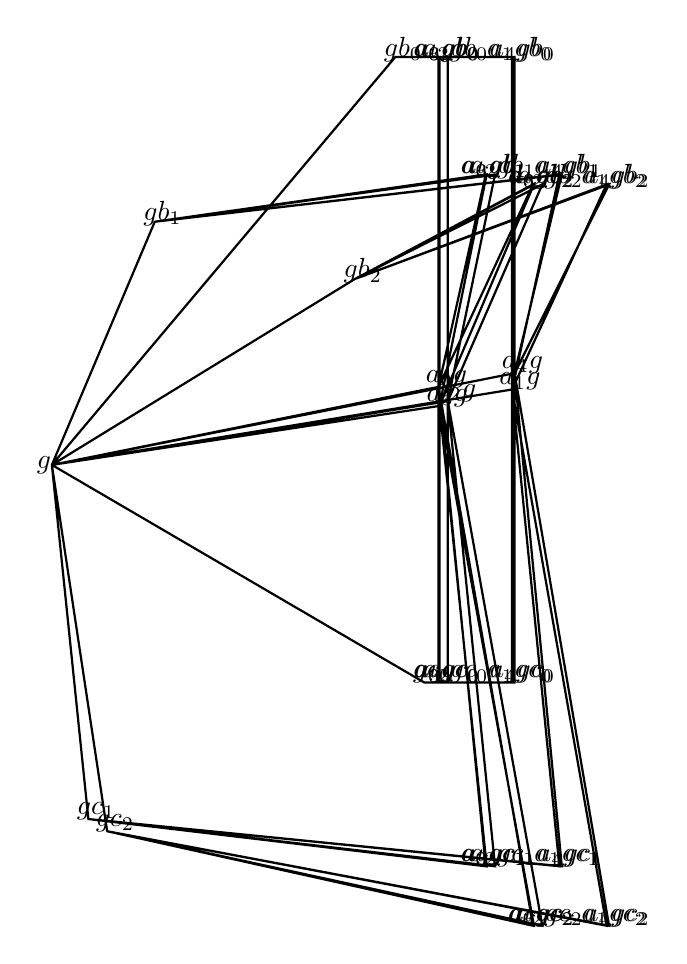
\begin{tikzpicture}
            \draw[thick](0,0)(0,0) -- (4.360919582359118,5.179444445290935) -- (4.910662039732638,5.179444445290935) -- (4.910662039732638,0.9910408025410982) -- (0,0)
(0,0) -- (1.3068588919511788,3.0880290222925675) -- (5.510662039732638,3.6880290222925676) -- (4.910662039732638,0.9910408025410982) -- (0,0)
(0,0) -- (3.8496719792024474,2.3618158465441828) -- (6.110662039732638,3.5618158465441825) -- (4.910662039732638,0.9910408025410982) -- (0,0)
(0,0) -- (4.360919582359118,5.179444445290935) -- (5.84475941047429,5.179444445290935) -- (5.84475941047429,0.9578399584119763) -- (0,0)
(0,0) -- (1.3068588919511788,3.0880290222925675) -- (6.44475941047429,3.6880290222925676) -- (5.84475941047429,0.9578399584119763) -- (0,0)
(0,0) -- (3.8496719792024474,2.3618158465441828) -- (7.04475941047429,3.5618158465441825) -- (5.84475941047429,0.9578399584119763) -- (0,0)
(0,0) -- (4.360919582359118,5.179444445290935) -- (5.0282379468287886,5.179444445290935) -- (5.0282379468287886,0.8095635731103051) -- (0,0)
(0,0) -- (1.3068588919511788,3.0880290222925675) -- (5.628237946828788,3.6880290222925676) -- (5.0282379468287886,0.8095635731103051) -- (0,0)
(0,0) -- (3.8496719792024474,2.3618158465441828) -- (6.228237946828789,3.5618158465441825) -- (5.0282379468287886,0.8095635731103051) -- (0,0)
(0,0) -- (4.360919582359118,5.179444445290935) -- (4.922306765800849,5.179444445290935) -- (4.922306765800849,0.7490074219057342) -- (0,0)
(0,0) -- (1.3068588919511788,3.0880290222925675) -- (5.522306765800849,3.6880290222925676) -- (4.922306765800849,0.7490074219057342) -- (0,0)
(0,0) -- (3.8496719792024474,2.3618158465441828) -- (6.122306765800849,3.5618158465441825) -- (4.922306765800849,0.7490074219057342) -- (0,0)
(0,0) -- (4.360919582359118,5.179444445290935) -- (5.876168714207703,5.179444445290935) -- (5.876168714207703,1.1648474061777094) -- (0,0)
(0,0) -- (1.3068588919511788,3.0880290222925675) -- (6.476168714207702,3.6880290222925676) -- (5.876168714207703,1.1648474061777094) -- (0,0)
(0,0) -- (3.8496719792024474,2.3618158465441828) -- (7.076168714207703,3.5618158465441825) -- (5.876168714207703,1.1648474061777094) -- (0,0)
(0,0) -- (4.73079901630061,-2.764104175734774) -- (4.910662039732638,-2.764104175734774) -- (4.910662039732638,0.9910408025410982) -- (0,0)
(0,0) -- (0.4637034706639226,-4.49732483184523) -- (5.510662039732638,-5.0973248318452296) -- (4.910662039732638,0.9910408025410982) -- (0,0)
(0,0) -- (0.7024436876713874,-4.65216696188478) -- (6.110662039732638,-5.85216696188478) -- (4.910662039732638,0.9910408025410982) -- (0,0)
(0,0) -- (4.73079901630061,-2.764104175734774) -- (5.84475941047429,-2.764104175734774) -- (5.84475941047429,0.9578399584119763) -- (0,0)
(0,0) -- (0.4637034706639226,-4.49732483184523) -- (6.44475941047429,-5.0973248318452296) -- (5.84475941047429,0.9578399584119763) -- (0,0)
(0,0) -- (0.7024436876713874,-4.65216696188478) -- (7.04475941047429,-5.85216696188478) -- (5.84475941047429,0.9578399584119763) -- (0,0)
(0,0) -- (4.73079901630061,-2.764104175734774) -- (5.0282379468287886,-2.764104175734774) -- (5.0282379468287886,0.8095635731103051) -- (0,0)
(0,0) -- (0.4637034706639226,-4.49732483184523) -- (5.628237946828788,-5.0973248318452296) -- (5.0282379468287886,0.8095635731103051) -- (0,0)
(0,0) -- (0.7024436876713874,-4.65216696188478) -- (6.228237946828789,-5.85216696188478) -- (5.0282379468287886,0.8095635731103051) -- (0,0)
(0,0) -- (4.73079901630061,-2.764104175734774) -- (4.922306765800849,-2.764104175734774) -- (4.922306765800849,0.7490074219057342) -- (0,0)
(0,0) -- (0.4637034706639226,-4.49732483184523) -- (5.522306765800849,-5.0973248318452296) -- (4.922306765800849,0.7490074219057342) -- (0,0)
(0,0) -- (0.7024436876713874,-4.65216696188478) -- (6.122306765800849,-5.85216696188478) -- (4.922306765800849,0.7490074219057342) -- (0,0)
(0,0) -- (4.73079901630061,-2.764104175734774) -- (5.876168714207703,-2.764104175734774) -- (5.876168714207703,1.1648474061777094) -- (0,0)
(0,0) -- (0.4637034706639226,-4.49732483184523) -- (6.476168714207702,-5.0973248318452296) -- (5.876168714207703,1.1648474061777094) -- (0,0)
(0,0) -- (0.7024436876713874,-4.65216696188478) -- (7.076168714207703,-5.85216696188478) -- (5.876168714207703,1.1648474061777094) -- (0,0)
;
\node at (5.010662039732638,5.279444445290935) {$ a_{ 0  } gb_{ 0 } $};
\node at (5.610662039732637,3.7880290222925677) {$ a_{ 0  } gb_{ 1 } $};
\node at (6.210662039732638,3.6618158465441826) {$ a_{ 0  } gb_{ 2 } $};
\node at (5.94475941047429,5.279444445290935) {$ a_{ 1  } gb_{ 0 } $};
\node at (6.544759410474289,3.7880290222925677) {$ a_{ 1  } gb_{ 1 } $};
\node at (7.14475941047429,3.6618158465441826) {$ a_{ 1  } gb_{ 2 } $};
\node at (5.128237946828788,5.279444445290935) {$ a_{ 2  } gb_{ 0 } $};
\node at (5.728237946828788,3.7880290222925677) {$ a_{ 2  } gb_{ 1 } $};
\node at (6.328237946828788,3.6618158465441826) {$ a_{ 2  } gb_{ 2 } $};
\node at (5.022306765800849,5.279444445290935) {$ a_{ 3  } gb_{ 0 } $};
\node at (5.6223067658008485,3.7880290222925677) {$ a_{ 3  } gb_{ 1 } $};
\node at (6.222306765800849,3.6618158465441826) {$ a_{ 3  } gb_{ 2 } $};
\node at (5.976168714207702,5.279444445290935) {$ a_{ 4  } gb_{ 0 } $};
\node at (6.576168714207702,3.7880290222925677) {$ a_{ 4  } gb_{ 1 } $};
\node at (7.176168714207702,3.6618158465441826) {$ a_{ 4  } gb_{ 2 } $};
\node at (5.010662039732638,-2.664104175734774) {$ a_{ 0  } gc_{ 0 } $};
\node at (5.610662039732637,-4.99732483184523) {$ a_{ 0  } gc_{ 1 } $};
\node at (6.210662039732638,-5.752166961884781) {$ a_{ 0  } gc_{ 2 } $};
\node at (5.94475941047429,-2.664104175734774) {$ a_{ 1  } gc_{ 0 } $};
\node at (6.544759410474289,-4.99732483184523) {$ a_{ 1  } gc_{ 1 } $};
\node at (7.14475941047429,-5.752166961884781) {$ a_{ 1  } gc_{ 2 } $};
\node at (5.128237946828788,-2.664104175734774) {$ a_{ 2  } gc_{ 0 } $};
\node at (5.728237946828788,-4.99732483184523) {$ a_{ 2  } gc_{ 1 } $};
\node at (6.328237946828788,-5.752166961884781) {$ a_{ 2  } gc_{ 2 } $};
\node at (5.022306765800849,-2.664104175734774) {$ a_{ 3  } gc_{ 0 } $};
\node at (5.6223067658008485,-4.99732483184523) {$ a_{ 3  } gc_{ 1 } $};
\node at (6.222306765800849,-5.752166961884781) {$ a_{ 3  } gc_{ 2 } $};
\node at (5.976168714207702,-2.664104175734774) {$ a_{ 4  } gc_{ 0 } $};
\node at (6.576168714207702,-4.99732483184523) {$ a_{ 4  } gc_{ 1 } $};
\node at (7.176168714207702,-5.752166961884781) {$ a_{ 4  } gc_{ 2 } $};
\node at (-0.1,0) {$ g $};
\node at (5.010662039732638,1.0910408025410983) {$ a_{ 0 }g $};
\node at (5.94475941047429,1.0578399584119764) {$ a_{ 1 }g $};
\node at (5.128237946828788,0.9095635731103051) {$ a_{ 2 }g $};
\node at (5.022306765800849,0.8490074219057342) {$ a_{ 3 }g $};
\node at (5.976168714207702,1.2648474061777095) {$ a_{ 4 }g $};
\node at (4.460919582359118,5.279444445290935) {$ gb_{ 0 } $};
\node at (1.4068588919511789,3.1880290222925676) {$ gb_{ 1 } $};
\node at (3.9496719792024475,2.461815846544183) {$ gb_{ 2 } $};
\node at (4.83079901630061,-2.664104175734774) {$ gc_{ 0 } $};
\node at (0.5637034706639226,-4.39732483184523) {$ gc_{ 1 } $};
\node at (0.8024436876713874,-4.55216696188478) {$ gc_{ 2 } $};

            \end{tikzpicture}
            \end{center}
            \caption{Square of the complex, with edges $(g,ag), (agb, gb) \in E_A,
            (g,gb), (agb, ag) \in E_B.$ \label{fig:square}
            }
            \end{figure}
 \begin{figure}[H]
            %\label{fig:square}
            \begin{center}
            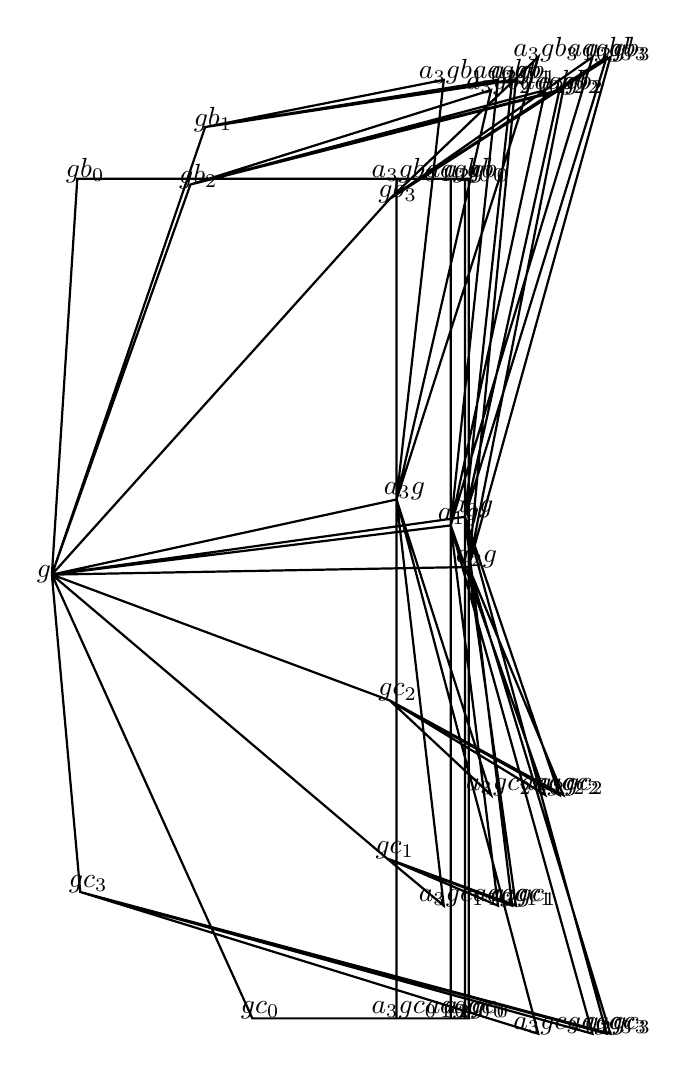
\begin{tikzpicture}
            \draw[thick](0,0)(0,0) -- (0.32306188553127,5.028767360934532) -- (5.24598901906943,5.028767360934532) -- (5.24598901906943,0.7339109629787509) -- (0,0)
(0,0) -- (1.946827070731079,5.683679905971232) -- (5.84598901906943,6.283679905971232) -- (5.24598901906943,0.7339109629787509) -- (0,0)
(0,0) -- (1.7597536907792484,4.954000635886928) -- (6.4459890190694304,6.154000635886928) -- (5.24598901906943,0.7339109629787509) -- (0,0)
(0,0) -- (4.292277057573047,4.772859316895506) -- (7.04598901906943,6.572859316895506) -- (5.24598901906943,0.7339109629787509) -- (0,0)
(0,0) -- (0.32306188553127,5.028767360934532) -- (5.065419469816285,5.028767360934532) -- (5.065419469816285,0.6248743617945312) -- (0,0)
(0,0) -- (1.946827070731079,5.683679905971232) -- (5.6654194698162845,6.283679905971232) -- (5.065419469816285,0.6248743617945312) -- (0,0)
(0,0) -- (1.7597536907792484,4.954000635886928) -- (6.265419469816285,6.154000635886928) -- (5.065419469816285,0.6248743617945312) -- (0,0)
(0,0) -- (4.292277057573047,4.772859316895506) -- (6.865419469816285,6.572859316895506) -- (5.065419469816285,0.6248743617945312) -- (0,0)
(0,0) -- (0.32306188553127,5.028767360934532) -- (5.293069949742218,5.028767360934532) -- (5.293069949742218,0.09670221648278265) -- (0,0)
(0,0) -- (1.946827070731079,5.683679905971232) -- (5.893069949742218,6.283679905971232) -- (5.293069949742218,0.09670221648278265) -- (0,0)
(0,0) -- (1.7597536907792484,4.954000635886928) -- (6.493069949742218,6.154000635886928) -- (5.293069949742218,0.09670221648278265) -- (0,0)
(0,0) -- (4.292277057573047,4.772859316895506) -- (7.093069949742218,6.572859316895506) -- (5.293069949742218,0.09670221648278265) -- (0,0)
(0,0) -- (0.32306188553127,5.028767360934532) -- (4.37710111671268,5.028767360934532) -- (4.37710111671268,0.9545583335810951) -- (0,0)
(0,0) -- (1.946827070731079,5.683679905971232) -- (4.97710111671268,6.283679905971232) -- (4.37710111671268,0.9545583335810951) -- (0,0)
(0,0) -- (1.7597536907792484,4.954000635886928) -- (5.57710111671268,6.154000635886928) -- (4.37710111671268,0.9545583335810951) -- (0,0)
(0,0) -- (4.292277057573047,4.772859316895506) -- (6.17710111671268,6.572859316895506) -- (4.37710111671268,0.9545583335810951) -- (0,0)
(0,0) -- (2.5460524181704725,-5.635505251664049) -- (5.24598901906943,-5.635505251664049) -- (5.24598901906943,0.7339109629787509) -- (0,0)
(0,0) -- (4.25530955904529,-3.60447268474004) -- (5.84598901906943,-4.20447268474004) -- (5.24598901906943,0.7339109629787509) -- (0,0)
(0,0) -- (4.2916497836572285,-1.5984521236749658) -- (6.4459890190694304,-2.7984521236749655) -- (5.24598901906943,0.7339109629787509) -- (0,0)
(0,0) -- (0.3606230992458942,-4.030457503586714) -- (7.04598901906943,-5.830457503586714) -- (5.24598901906943,0.7339109629787509) -- (0,0)
(0,0) -- (2.5460524181704725,-5.635505251664049) -- (5.065419469816285,-5.635505251664049) -- (5.065419469816285,0.6248743617945312) -- (0,0)
(0,0) -- (4.25530955904529,-3.60447268474004) -- (5.6654194698162845,-4.20447268474004) -- (5.065419469816285,0.6248743617945312) -- (0,0)
(0,0) -- (4.2916497836572285,-1.5984521236749658) -- (6.265419469816285,-2.7984521236749655) -- (5.065419469816285,0.6248743617945312) -- (0,0)
(0,0) -- (0.3606230992458942,-4.030457503586714) -- (6.865419469816285,-5.830457503586714) -- (5.065419469816285,0.6248743617945312) -- (0,0)
(0,0) -- (2.5460524181704725,-5.635505251664049) -- (5.293069949742218,-5.635505251664049) -- (5.293069949742218,0.09670221648278265) -- (0,0)
(0,0) -- (4.25530955904529,-3.60447268474004) -- (5.893069949742218,-4.20447268474004) -- (5.293069949742218,0.09670221648278265) -- (0,0)
(0,0) -- (4.2916497836572285,-1.5984521236749658) -- (6.493069949742218,-2.7984521236749655) -- (5.293069949742218,0.09670221648278265) -- (0,0)
(0,0) -- (0.3606230992458942,-4.030457503586714) -- (7.093069949742218,-5.830457503586714) -- (5.293069949742218,0.09670221648278265) -- (0,0)
(0,0) -- (2.5460524181704725,-5.635505251664049) -- (4.37710111671268,-5.635505251664049) -- (4.37710111671268,0.9545583335810951) -- (0,0)
(0,0) -- (4.25530955904529,-3.60447268474004) -- (4.97710111671268,-4.20447268474004) -- (4.37710111671268,0.9545583335810951) -- (0,0)
(0,0) -- (4.2916497836572285,-1.5984521236749658) -- (5.57710111671268,-2.7984521236749655) -- (4.37710111671268,0.9545583335810951) -- (0,0)
(0,0) -- (0.3606230992458942,-4.030457503586714) -- (6.17710111671268,-5.830457503586714) -- (4.37710111671268,0.9545583335810951) -- (0,0)
;
\node at (5.34598901906943,5.128767360934532) {$ a_{ 0  } gb_{ 0 } $};
\node at (5.94598901906943,6.383679905971231) {$ a_{ 0  } gb_{ 1 } $};
\node at (6.54598901906943,6.254000635886928) {$ a_{ 0  } gb_{ 2 } $};
\node at (7.14598901906943,6.672859316895505) {$ a_{ 0  } gb_{ 3 } $};
\node at (5.1654194698162845,5.128767360934532) {$ a_{ 1  } gb_{ 0 } $};
\node at (5.765419469816284,6.383679905971231) {$ a_{ 1  } gb_{ 1 } $};
\node at (6.365419469816285,6.254000635886928) {$ a_{ 1  } gb_{ 2 } $};
\node at (6.965419469816284,6.672859316895505) {$ a_{ 1  } gb_{ 3 } $};
\node at (5.393069949742218,5.128767360934532) {$ a_{ 2  } gb_{ 0 } $};
\node at (5.9930699497422175,6.383679905971231) {$ a_{ 2  } gb_{ 1 } $};
\node at (6.593069949742218,6.254000635886928) {$ a_{ 2  } gb_{ 2 } $};
\node at (7.193069949742218,6.672859316895505) {$ a_{ 2  } gb_{ 3 } $};
\node at (4.47710111671268,5.128767360934532) {$ a_{ 3  } gb_{ 0 } $};
\node at (5.077101116712679,6.383679905971231) {$ a_{ 3  } gb_{ 1 } $};
\node at (5.67710111671268,6.254000635886928) {$ a_{ 3  } gb_{ 2 } $};
\node at (6.27710111671268,6.672859316895505) {$ a_{ 3  } gb_{ 3 } $};
\node at (5.34598901906943,-5.535505251664049) {$ a_{ 0  } gc_{ 0 } $};
\node at (5.94598901906943,-4.10447268474004) {$ a_{ 0  } gc_{ 1 } $};
\node at (6.54598901906943,-2.6984521236749655) {$ a_{ 0  } gc_{ 2 } $};
\node at (7.14598901906943,-5.730457503586714) {$ a_{ 0  } gc_{ 3 } $};
\node at (5.1654194698162845,-5.535505251664049) {$ a_{ 1  } gc_{ 0 } $};
\node at (5.765419469816284,-4.10447268474004) {$ a_{ 1  } gc_{ 1 } $};
\node at (6.365419469816285,-2.6984521236749655) {$ a_{ 1  } gc_{ 2 } $};
\node at (6.965419469816284,-5.730457503586714) {$ a_{ 1  } gc_{ 3 } $};
\node at (5.393069949742218,-5.535505251664049) {$ a_{ 2  } gc_{ 0 } $};
\node at (5.9930699497422175,-4.10447268474004) {$ a_{ 2  } gc_{ 1 } $};
\node at (6.593069949742218,-2.6984521236749655) {$ a_{ 2  } gc_{ 2 } $};
\node at (7.193069949742218,-5.730457503586714) {$ a_{ 2  } gc_{ 3 } $};
\node at (4.47710111671268,-5.535505251664049) {$ a_{ 3  } gc_{ 0 } $};
\node at (5.077101116712679,-4.10447268474004) {$ a_{ 3  } gc_{ 1 } $};
\node at (5.67710111671268,-2.6984521236749655) {$ a_{ 3  } gc_{ 2 } $};
\node at (6.27710111671268,-5.730457503586714) {$ a_{ 3  } gc_{ 3 } $};
\node at (-0.1,0) {$ g $};
\node at (5.34598901906943,0.8339109629787509) {$ a_{ 0 }g $};
\node at (5.1654194698162845,0.7248743617945311) {$ a_{ 1 }g $};
\node at (5.393069949742218,0.19670221648278266) {$ a_{ 2 }g $};
\node at (4.47710111671268,1.054558333581095) {$ a_{ 3 }g $};
\node at (0.42306188553127,5.128767360934532) {$ gb_{ 0 } $};
\node at (2.046827070731079,5.783679905971232) {$ gb_{ 1 } $};
\node at (1.8597536907792485,5.054000635886927) {$ gb_{ 2 } $};
\node at (4.392277057573047,4.872859316895505) {$ gb_{ 3 } $};
\node at (2.6460524181704725,-5.535505251664049) {$ gc_{ 0 } $};
\node at (4.355309559045289,-3.50447268474004) {$ gc_{ 1 } $};
\node at (4.391649783657228,-1.4984521236749657) {$ gc_{ 2 } $};
\node at (0.4606230992458942,-3.9304575035867138) {$ gc_{ 3 } $};

            \end{tikzpicture}
            \end{center}
            \caption{Square of the complex, with edges $(g,ag), (agb, gb) \in E_A,
            (g,gb), (agb, ag) \in E_B.$ \label{fig:square}
            }
            \end{figure}
 
%\end{multicols*}
  % \printbibliography 
\end{document}

 